% A LaTeX template for MSc Thesis submissions to 
% Politecnico di Milano (PoliMi) - School of Industrial and Information Engineering
%
% S. Bonetti, A. Gruttadauria, G. Mescolini, A. Zingaro
% e-mail: template-tesi-ingind@polimi.it
%
% Last Revision: October 2021
%
% Copyright 2021 Politecnico di Milano, Italy. NC-BY

\documentclass{Configuration_Files/PoliMi3i_thesis}

%------------------------------------------------------------------------------
%   REQUIRED PACKAGES AND  CONFIGURATIONS
%------------------------------------------------------------------------------

% CONFIGURATIONS
\usepackage{parskip} % For paragraph layout
\usepackage{setspace} % For using single or double spacing
\usepackage{emptypage} % To insert empty pages
\usepackage{multicol} % To write in multiple columns (executive summary)
\setlength\columnsep{15pt} % Column separation in executive summary
\setlength\parindent{0pt} % Indentation
\raggedbottom  

% PACKAGES FOR TITLES
\usepackage{titlesec}
% \titlespacing{\section}{left spacing}{before spacing}{after spacing}
\titlespacing{\section}{0pt}{3.3ex}{2ex}
\titlespacing{\subsection}{0pt}{3.3ex}{1.65ex}
\titlespacing{\subsubsection}{0pt}{3.3ex}{1ex}
\usepackage{color}

% PACKAGES FOR LANGUAGE AND FONT
\usepackage[english]{babel} % The document is in English  
\usepackage[utf8]{inputenc} % UTF8 encoding
\usepackage[T1]{fontenc} % Font encoding
\usepackage[11pt]{moresize} % Big fonts

% PACKAGES FOR IMAGES
\usepackage{graphicx}
\usepackage{transparent} % Enables transparent images
\usepackage{eso-pic} % For the background picture on the title page
\usepackage{subfig} % Numbered and caption subfigures using \subfloat.
\usepackage{tikz} % A package for high-quality hand-made figures.
\usetikzlibrary{}
\graphicspath{{./Images/}} % Directory of the images
\usepackage{caption} % Coloured captions
\usepackage{xcolor} % Coloured captions
\usepackage{amsthm,thmtools,xcolor} % Coloured "Theorem"
\usepackage{float}

% STANDARD MATH PACKAGES
\usepackage{amsmath}
\usepackage{amsthm}
\usepackage{amssymb}
\usepackage{amsfonts}
\usepackage{bm}
\usepackage[overload]{empheq} % For braced-style systems of equations.
\usepackage{fix-cm} % To override original LaTeX restrictions on sizes
\usepackage{siunitx}

% PACKAGES FOR TABLES
\usepackage{tabularx}
\usepackage{longtable} % Tables that can span several pages
\usepackage{colortbl}

% PACKAGES FOR ALGORITHMS (PSEUDO-CODE)
\usepackage{algorithm}
\usepackage{algorithmic}

% PACKAGES FOR CODE
\usepackage[outputdir=.texpadtmp]{minted}

% PACKAGES FOR REFERENCES & BIBLIOGRAPHY
\usepackage[colorlinks=true,linkcolor=bluepoli,anchorcolor=black,citecolor=black,filecolor=black,menucolor=black,runcolor=black,urlcolor=black]{hyperref} % Adds clickable links at references
\usepackage{cleveref}
\usepackage[square, numbers, sort&compress]{natbib} % Square brackets, citing references with numbers, citations sorted by appearance in the text and compressed
\bibliographystyle{abbrvnat} % You may use a different style adapted to your field

% OTHER PACKAGES
\usepackage{pdfpages} % To include a pdf file
\usepackage{afterpage}
\usepackage{lipsum} % DUMMY PACKAGE
\usepackage{fancyhdr} % For the headers
\fancyhf{}

% Input of configuration file. Do not change config.tex file unless you really know what you are doing. 
% Define blue color typical of polimi
\definecolor{bluepoli}{cmyk}{0.4,0.1,0,0.4}

% Custom theorem environments
\declaretheoremstyle[
  headfont=\color{bluepoli}\normalfont\bfseries,
  bodyfont=\color{black}\normalfont\itshape,
]{colored}

% Set-up caption colors
\captionsetup[figure]{labelfont={color=bluepoli}} % Set colour of the captions
\captionsetup[table]{labelfont={color=bluepoli}} % Set colour of the captions
\captionsetup[algorithm]{labelfont={color=bluepoli}} % Set colour of the captions

\theoremstyle{colored}
\newtheorem{theorem}{Theorem}[chapter]
\newtheorem{proposition}{Proposition}[chapter]

% Enhances the features of the standard "table" and "tabular" environments.
\newcommand\T{\rule{0pt}{2.6ex}}
\newcommand\B{\rule[-1.2ex]{0pt}{0pt}}

% Pseudo-code algorithm descriptions.
\newcounter{algsubstate}
\renewcommand{\thealgsubstate}{\alph{algsubstate}}
\newenvironment{algsubstates}
  {\setcounter{algsubstate}{0}%
   \renewcommand{\STATE}{%
     \stepcounter{algsubstate}%
     \Statex {\small\thealgsubstate:}\space}}
  {}

% New font size
\newcommand\numfontsize{\@setfontsize\Huge{200}{60}}

% Title format: chapter
\titleformat{\chapter}[hang]{
\fontsize{50}{20}\selectfont\bfseries\filright}{\textcolor{bluepoli} \thechapter\hsp\hspace{2mm}\textcolor{bluepoli}{|   }\hsp}{0pt}{\huge\bfseries \textcolor{bluepoli}
}

% Title format: section
\titleformat{\section}
{\color{bluepoli}\normalfont\Large\bfseries}
{\color{bluepoli}\thesection.}{1em}{}

% Title format: subsection
\titleformat{\subsection}
{\color{bluepoli}\normalfont\large\bfseries}
{\color{bluepoli}\thesubsection.}{1em}{}

% Title format: subsubsection
\titleformat{\subsubsection}
{\color{bluepoli}\normalfont\large\bfseries}
{\color{bluepoli}\thesubsubsection.}{1em}{}

% Shortening for setting no horizontal-spacing
\newcommand{\hsp}{\hspace{0pt}}

\makeatletter

%For correctly numbering algorithms
\numberwithin{algorithm}{chapter}

%----------------------------------------------------------------------------
%   NEW COMMANDS DEFINED
%----------------------------------------------------------------------------

% EXAMPLES OF NEW COMMANDS
\newcommand{\bea}{\begin{eqnarray}} % Shortcut for equation arrays
\newcommand{\eea}{\end{eqnarray}}
\newcommand{\e}[1]{\times 10^{#1}}  % Powers of 10 notation

%----------------------------------------------------------------------------
%   ADD YOUR PACKAGES (be careful of package interaction)
%----------------------------------------------------------------------------

%----------------------------------------------------------------------------
%   ADD YOUR DEFINITIONS AND COMMANDS (be careful of existing commands)
%----------------------------------------------------------------------------

%----------------------------------------------------------------------------
%   BEGIN OF YOUR DOCUMENT
%----------------------------------------------------------------------------

\begin{document}

\fancypagestyle{plain}{%
\fancyhf{} % Clear all header and footer fields
\fancyhead[RO,RE]{\thepage} %RO=right odd, RE=right even
\renewcommand{\headrulewidth}{0pt}
\renewcommand{\footrulewidth}{0pt}}

%----------------------------------------------------------------------------
%   TITLE PAGE
%----------------------------------------------------------------------------

\pagestyle{empty} % No page numbers
\frontmatter % Use roman page numbering style (i, ii, iii, iv...) for the preamble pages

\puttitle{
    title=Homework Report, % Title of the thesis
    name=Christian Grasso, % Author Name and Surname
    ID = 10652464,
    course=Image Analysis and Computer Vision,
    academicyear={2021-22},  % Academic Year
} % These info will be put into your Title page 

%----------------------------------------------------------------------------
%   PREAMBLE PAGES: ABSTRACT (inglese e italiano), EXECUTIVE SUMMARY
%----------------------------------------------------------------------------
\startpreamble
\setcounter{page}{1} % Set page counter to 1

%----------------------------------------------------------------------------
%   LIST OF CONTENTS/FIGURES/TABLES/SYMBOLS
%----------------------------------------------------------------------------

% TABLE OF CONTENTS
\thispagestyle{empty}
{\hypersetup{linkcolor=black}
\tableofcontents % Table of contents
}
\thispagestyle{empty}

%-------------------------------------------------------------------------
%   THESIS MAIN TEXT
%-------------------------------------------------------------------------
% In the main text of your thesis you can write the chapters in two different ways:
%
%(1) As presented in this template you can write:
%    \chapter{Title of the chapter}
%    *body of the chapter*
%
%(2) You can write your chapter in a separated .tex file and then include it in the main file with the following command:
%    \chapter{Title of the chapter}
%    \input{chapter_file.tex}
%
% Especially for long thesis, we recommend you the second option.

\addtocontents{toc}{\vspace{2em}} % Add a gap in the Contents, for aesthetics
\mainmatter % Begin numeric (1,2,3...) page numbering

% --------------------------------------------------------------------------
% NUMBERED CHAPTERS % Regular chapters following
% --------------------------------------------------------------------------
\chapter{Introduction}

This is the report for the Image Analysis and Computer Vision Homework, A.Y. 2021-22.
The assignment consisted in processing an image of Villa Melzi d'Eril in Bellagio, analyzing its geometry and performing 2D reconstruction.
\section{Used Matlab functions}
Throughout the Matlab program, various functions were used, including some custom functions. The full code for the used functions can be found in the \verb|functions| folder in the delivered zip files, and in \hyperref[appendix:functions]{Appendix A}.

\begin{itemize}
\item \verb|segToLine(pts)| (as seen in class)\newline
Convert the endpoints of a line segment to a line in homogeneous coordinates (\verb|pts = [x1 y1; x2 y2]|)
\item \verb|fitLine(XY)| (as seen in class)\newline
Least squares fit of a line to a set of points. \verb|XY| is a \verb|2xN| array of xy coordinates.
\item \verb|drawLineFamilies(title, nFamilies, nLinesPerFamily)|\newline
Ask the user to draw \verb|nFamilies| families of \verb|nLinesPerFamily| segments, and return a \verb|nFamilies x 1| cell with lines in homogeneous coordinates.
\item \verb|drawLines(title_, nLines, color)|\newline
Ask the user to draw \verb|nLinesPerFamily| segments, and return a \verb|nLines x 3| vector with lines in homogeneous coordinates.
\item \verb|hpnorm(p)|\newline
Normalize a homogeneous coordinates vector representing a point.
\newpage
\item \verb|buildHaff(lines)|\newline
Build an affine rectification matrix using the specified line families (\verb|lines| is usually the output of \verb|drawLineFamilies|)
\item \verb|buildRotationMatrix(angle)|\newline
Build a rotation matrix for the specified angle (in radians).
\end{itemize}


\chapter{F1 - Feature extraction}
\label{ch:f1}%

The objective is to find edges, corner features and straight lines in the image.

\section{Edge detection}
\label{section:f1:edge_detection}
The \textbf{Canny} method can be used to detect edges in the image. The algorithm works by first applying a smoothing Gaussian filter to the image (to remove noise), then computing the gradient of the image, applying nonmax suppression and tracking edges via hysteresis thresholding.

Matlab already includes (in the Image Processing Toolbox) an implementation for this method in the \verb|edge| function.

First, we need to convert the image to grayscale. This way, the resulting image matrix will contain \verb|double|s in the $[0,1]$ interval, representing the "intensity" of each pixel.

\begin{minted}{matlab}
img = im2double(imread('villa.png'));
imgGrayscale = rgb2gray(img);
\end{minted}

Then we can simply use the \verb|edge| function to apply the Canny method. A threshold can be specified to adjust the output image; in this case a value of \verb|[0, 0.1]| seems to yield the best results.
\begin{minted}{matlab}
edges = edge(imgGrayscale, 'canny', [0 0.1]);
\end{minted}

The output image is fairly good, but it is a bit too noisy for the subsequent step of detecting straight lines. We can either try to reduce the threshold, which however seems to cut a lot of "good" lines from the output, or scale the image down to reduce detail:

\begin{minted}{matlab}
resizeMult = 0.6;
newSize = resizeMult.*size(img, [1 2]);
imgGrayscaleRescaled = imresize(imgGrayscale, newSize, 'bilinear');
imgRescaled = imresize(img, newSize, 'bilinear');
\end{minted}

\begin{figure}[H]
    \centering
    \subfloat[Canny at 100\% scale\label{fig:f1_canny_def}]{
        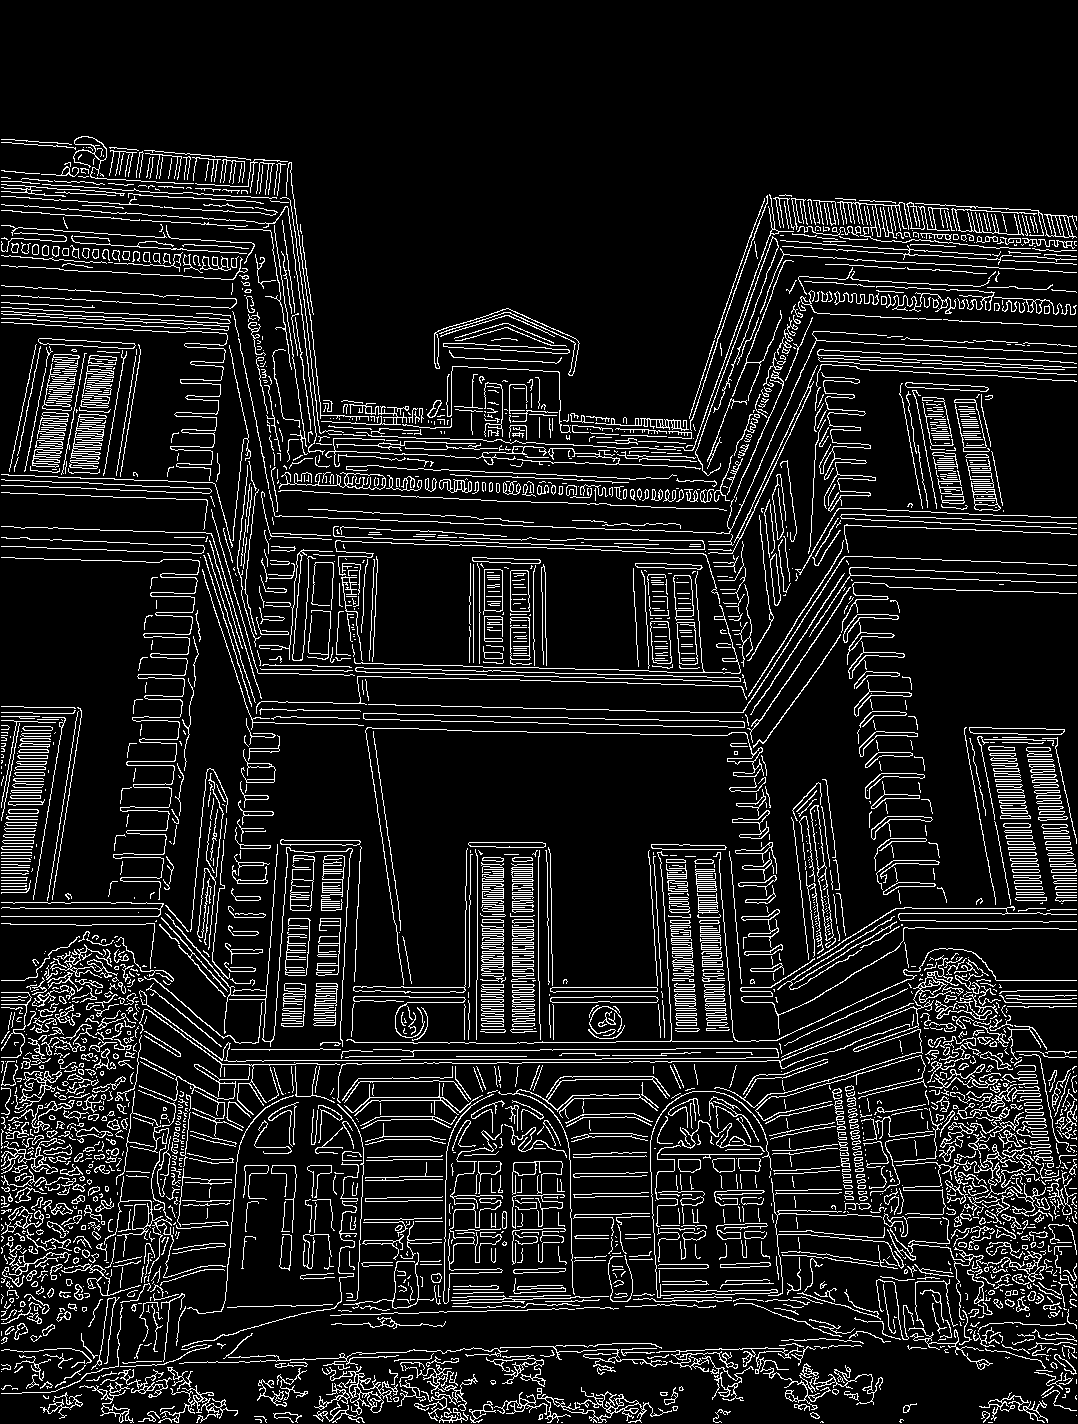
\includegraphics[scale=0.16]{output/F1_edges_100.PNG}
    }
    \quad
    \subfloat[Canny at 50\% scale\label{fig:f1_canny_85}]{
        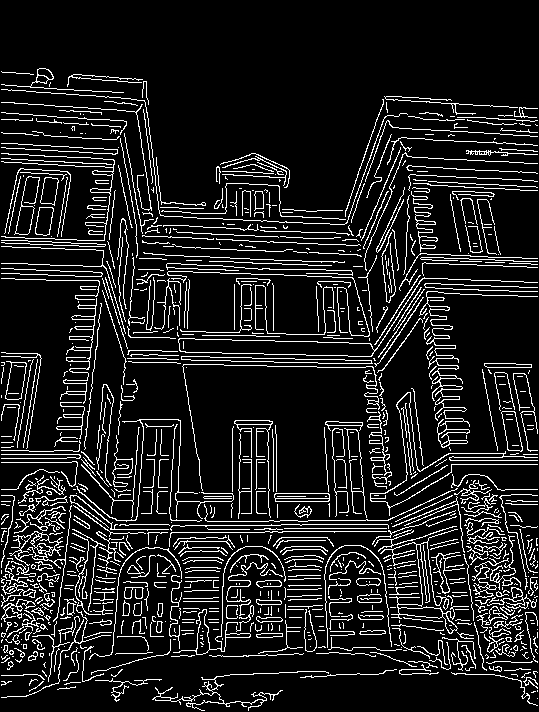
\includegraphics[scale=0.32]{output/F1_edges_50.PNG}
    }
    \caption[Output of Canny edge detection]{Output of Canny edge detection}
    \label{fig:quadtree2}
\end{figure}

\section{Straight line detection}
\label{section:f1:straight_line_detection}

We can use the results of the previous step to detect straight lines in the image. This can be done using the \textbf{Hough transform}. A Hough transform of a datum (in this case a point on a detected edge) is a set of models compatible with the datum in the \emph{model space}.
For a point in the cartesian plane, the HT will be a sinusoid; collinear points will map to (almost) concurrent HTs.

The Hough transform is also included in Matlab:
\begin{minted}{matlab}
[H,T,R] = hough(edges);
\end{minted}
where \verb|T| is $\theta$, \verb|R| is $\rho$ and \verb|H| is a matrix whose rows and columns correspond to $\rho$ and $\theta$ values respectively.

We can then use the \verb|houghpeaks| function to detect peaks, and pass the results to \verb|houghlines| to extract lines.
\newpage
\begin{minted}{matlab}
P = houghpeaks(H, 100, 'threshold', 0.3*max(H(:)));
hlines = houghlines(edges, T, R, P, 'FillGap', 4, 'MinLength', 14);
\end{minted}

These functions include various configuration options, namely:
\begin{itemize}
	\item \verb|numpeaks| is the number of peaks to detect (set to 100 here)
	\item \verb|threshold| is the minimum value to be considered a peak. By default it is set to half the maximum value in the \verb|H| matrix. For our image, we can get better results by lowering it to 30\% of the max value.
	\item \verb|FillGap| is, quoting the Matlab documentation, \emph{the distance between two line segments associated with the same Hough transform bin}. In practice, this value controls the max distance between two detected segments for them to be merged into one segment.
	\item \verb|MinLength| controls the minimum length for a segment. Setting this to a higher value allows to remove some bad segments in noisy areas of the image (e.g. the hedge).
\end{itemize}

\begin{figure}[H]
    \centering
    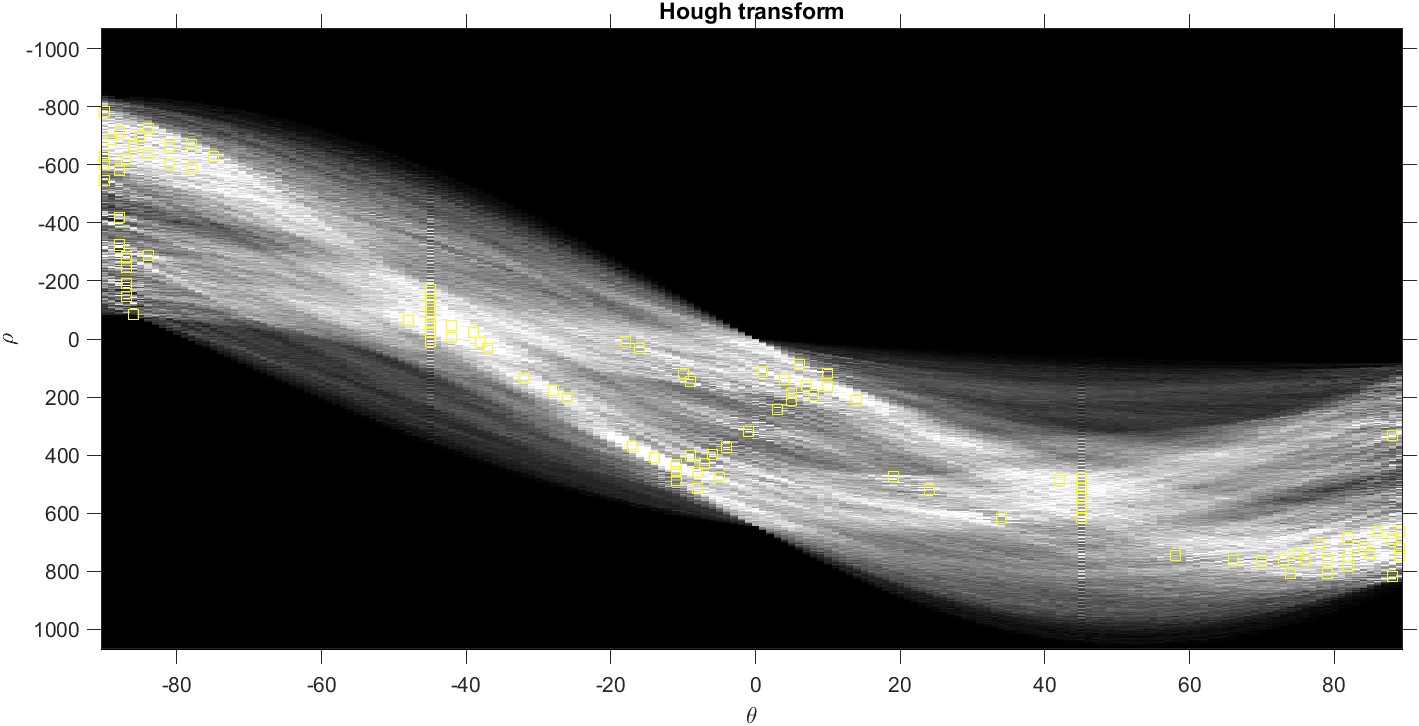
\includegraphics[width=0.9\textwidth]{output/F1_hough_peaks.png}
    \caption{Hough Transform and detected peaks (yellow) for the image}
    \label{fig:f1_hough_peaks}
\end{figure}
\newpage

The parameters detailed above can be adjusted based on whether we want a cleaner output or more/longer lines in the output.

\begin{figure}[H]
    \centering
    \subfloat[peaks=100, FillGaps=4, MinLength=14\label{fig:f1_hough_lines_1}]{
        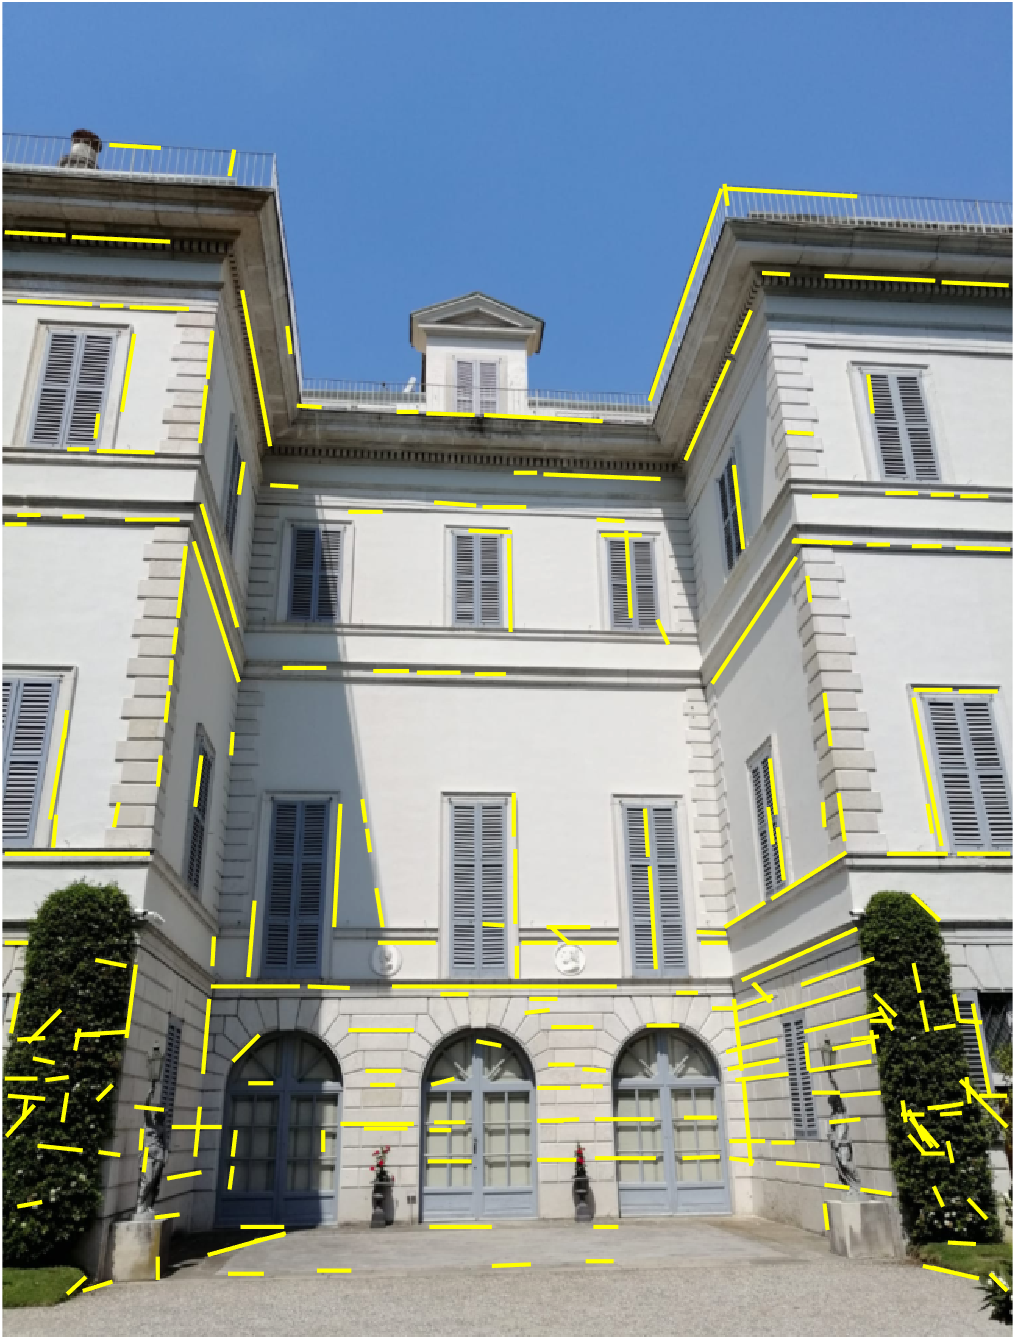
\includegraphics[scale=0.4]{output/F1_hough_n100_fg4_ml14.PNG}
    }
    \quad
    \subfloat[peaks=40, FillGaps=8, MinLength=10\label{fig:f1_hough_lines_2}]{
        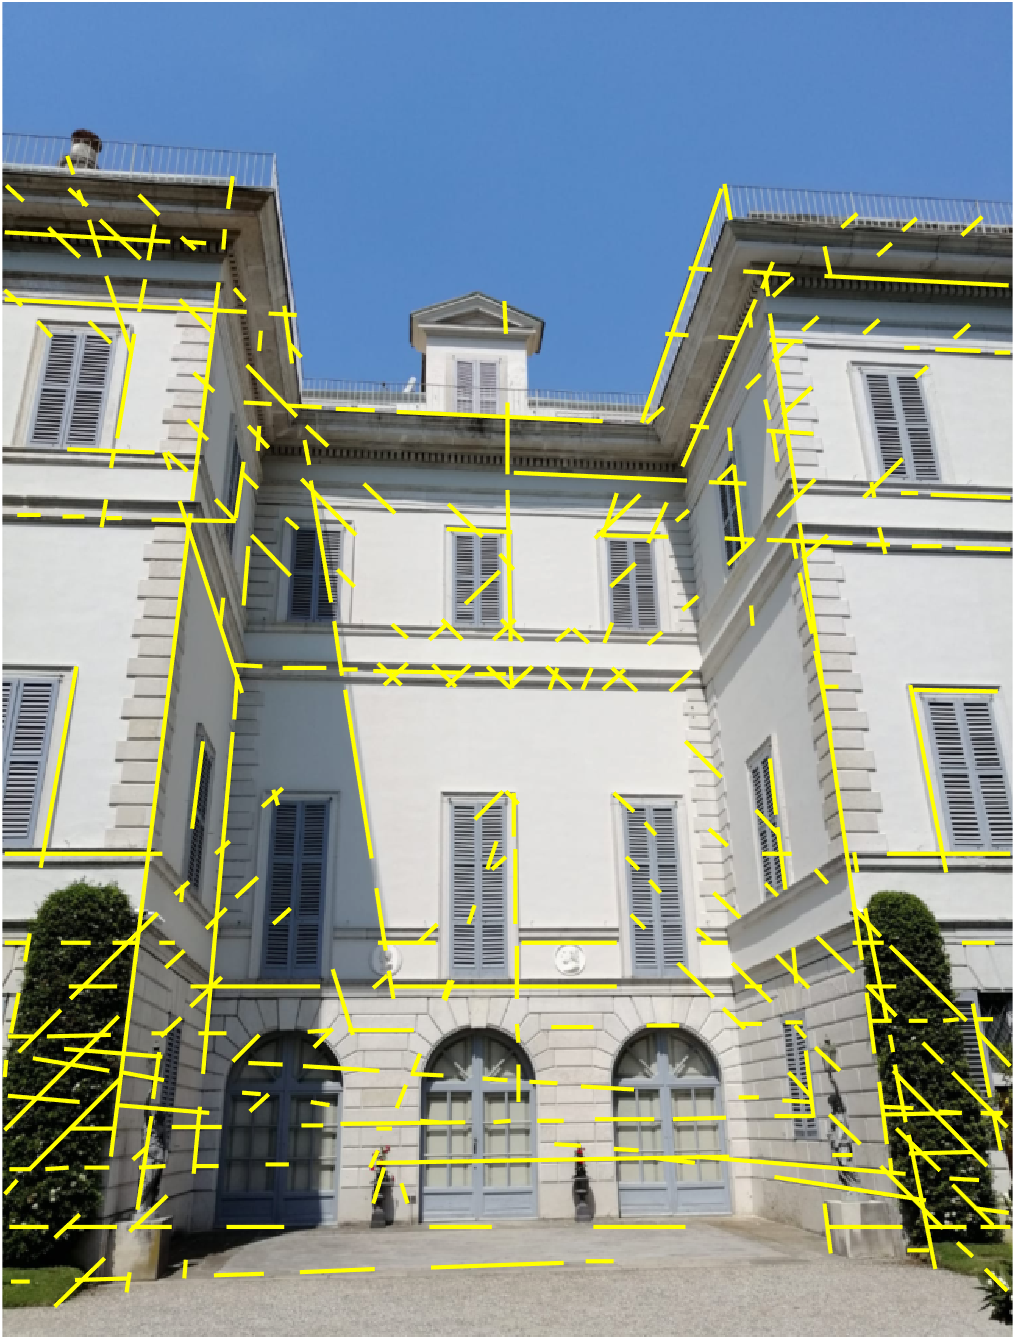
\includegraphics[scale=0.4]{output/F1_hough_n40_fg8_ml10.PNG}
    }
    \caption[Straight lines detected with the Hough Transform]{Straight lines detected with the Hough Transform}
    \label{fig:f1_hough_lines}
\end{figure}

\section{Corner detection}

We are going to use the \textbf{Harris-Stephens} corner detection algorithm. This algorithm is based on Moravac's corner detector, which works by splitting the image in small \emph{patches} of pixels, and checking how much a patch differs to the surrounding patches. If significant changes are present in both directions, the patch being analyzed is possibly a corner.

Matlab implements this algorithm in the Computer Vision Toolbox, and we can easily apply it to our image:

\begin{minted}{matlab}
points = detectHarrisFeatures(imgGrayscale);
figure; imshow(img); hold all;
plot(points.selectStrongest(5000));
\end{minted}
\newpage

The detection already works rather well without any adjustment, however not all corners are being detected and there are a lot of points in noisy areas like the hedge.

We can try to tackle this problem by increasing the contrast of the image, which should increase the differences for actual corners and push down the score of noisy areas.
One way to do this is using the \verb|histeq| function, which implements \textbf{histogram equalization}, a method that spreads the contrast values in the image between the minimum and maximum possible values (since our image is grayscale, this means the darkest pixels will be black and the brightest will be white).

This yields a way better result with a larger number of real corners being detected (e.g. in the railing) and fewer "wrong" points.

\begin{figure}[H]
    \centering
    \subfloat[No equalization\label{fig:f1_harris_}]{
        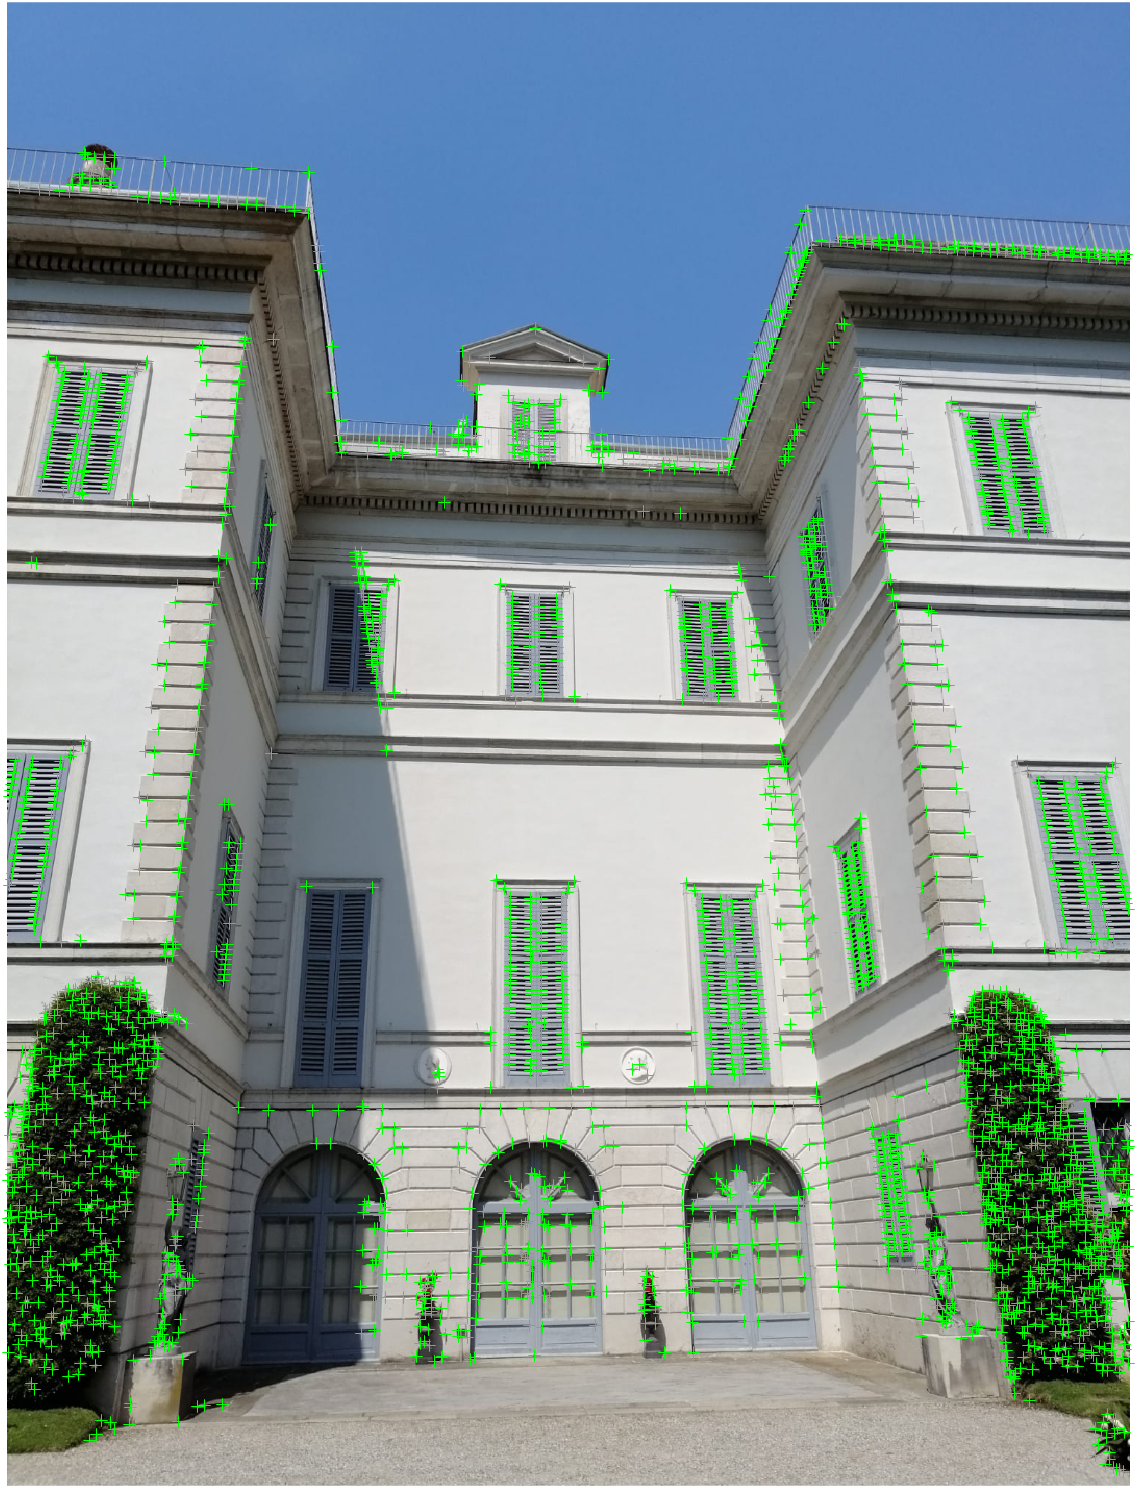
\includegraphics[width=0.45\textwidth]{output/F1_harris_noeq.png}
    }
    \quad
    \subfloat[Histogram equalization applied\label{fig:}]{
        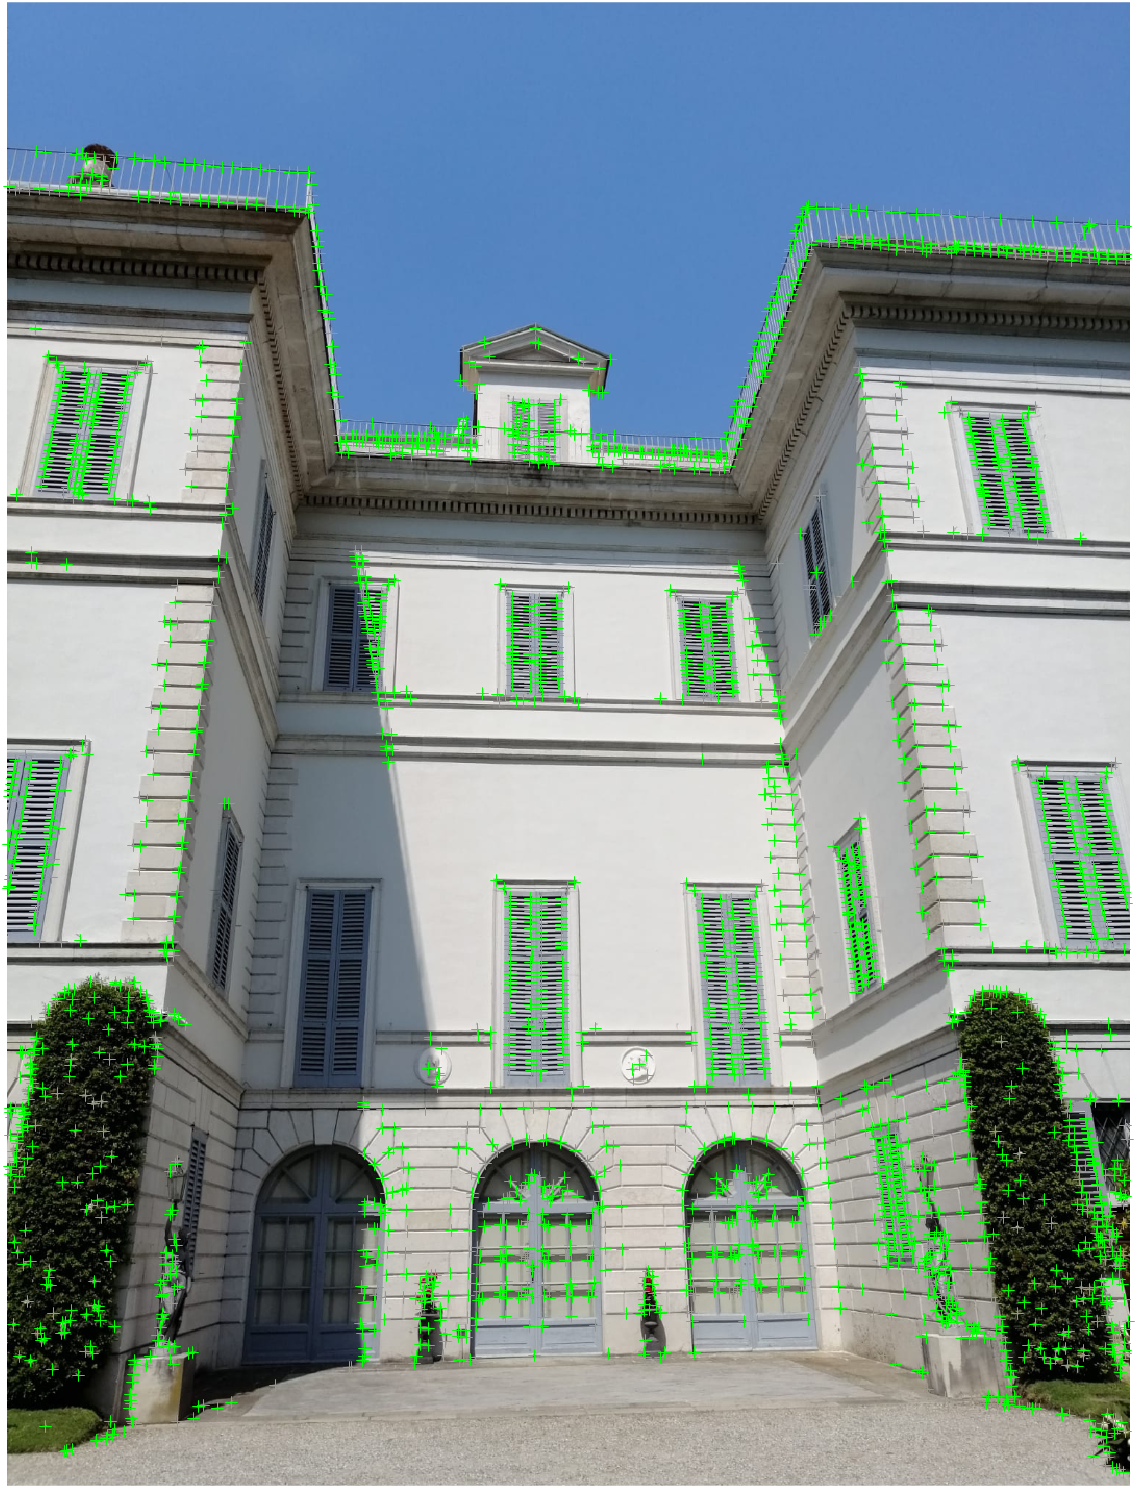
\includegraphics[width=0.45\textwidth]{output/F1_harris_histeq.png}
    }
    \caption{Harris-Stephens corner detection results}
    \label{fig:f1_harris}
\end{figure}

\chapter{G1 - 2D reconstruction of a horizontal section}
\label{ch:g1}

The objective is to metric rectify (2D reconstruct) the horizontal section of the Villa, and to determine the ratio between the side facades (numbered 2 and 4) and the center facade (number 3). The calibration matrix is unknown at this point.

In order to compute the rectifiying homography $H_rect$, we need to compute the \emph{image of the conic dual to the circular points} $C^{*'}_\infty$. One way to do this is using the so-called \textbf{stratified method}, which consists of first performing an \textbf{affine rectification} and then finding $C^{*'}_\infty$ through two more constraints (e.g. lines at a known angle).

\section{Affine rectification}
To perform affine rectification, we need at least two families of parallel lines, but we can use more to improve accuracy. In my case, three families were used. The lines are manually selected by the user on the image, as the lines detected in \ref{section:f1:straight_line_detection} were not accurate enough to obtain acceptable results.

\begin{minted}{matlab}
figure;
hold all;
imshow(img);

nFamilies = 3;
parallelLines = drawLineFamilies('Draw parallel lines', nFamilies, 2);
\end{minted}

We then build the affine rectification matrix using the \verb|buildHaff| function, which also returns the image of the line at infinity. The function internally uses \verb|fitLine|, which uses least squares to find the vanishing points of each direction.

\begin{minted}{matlab}
[H_aff, imHLinf] = buildHaff(parallelLines);
\end{minted}

\begin{figure}[H]
    \centering
    \subfloat[Lines used for affine rectification\label{fig:g1_affine_lines}]{
        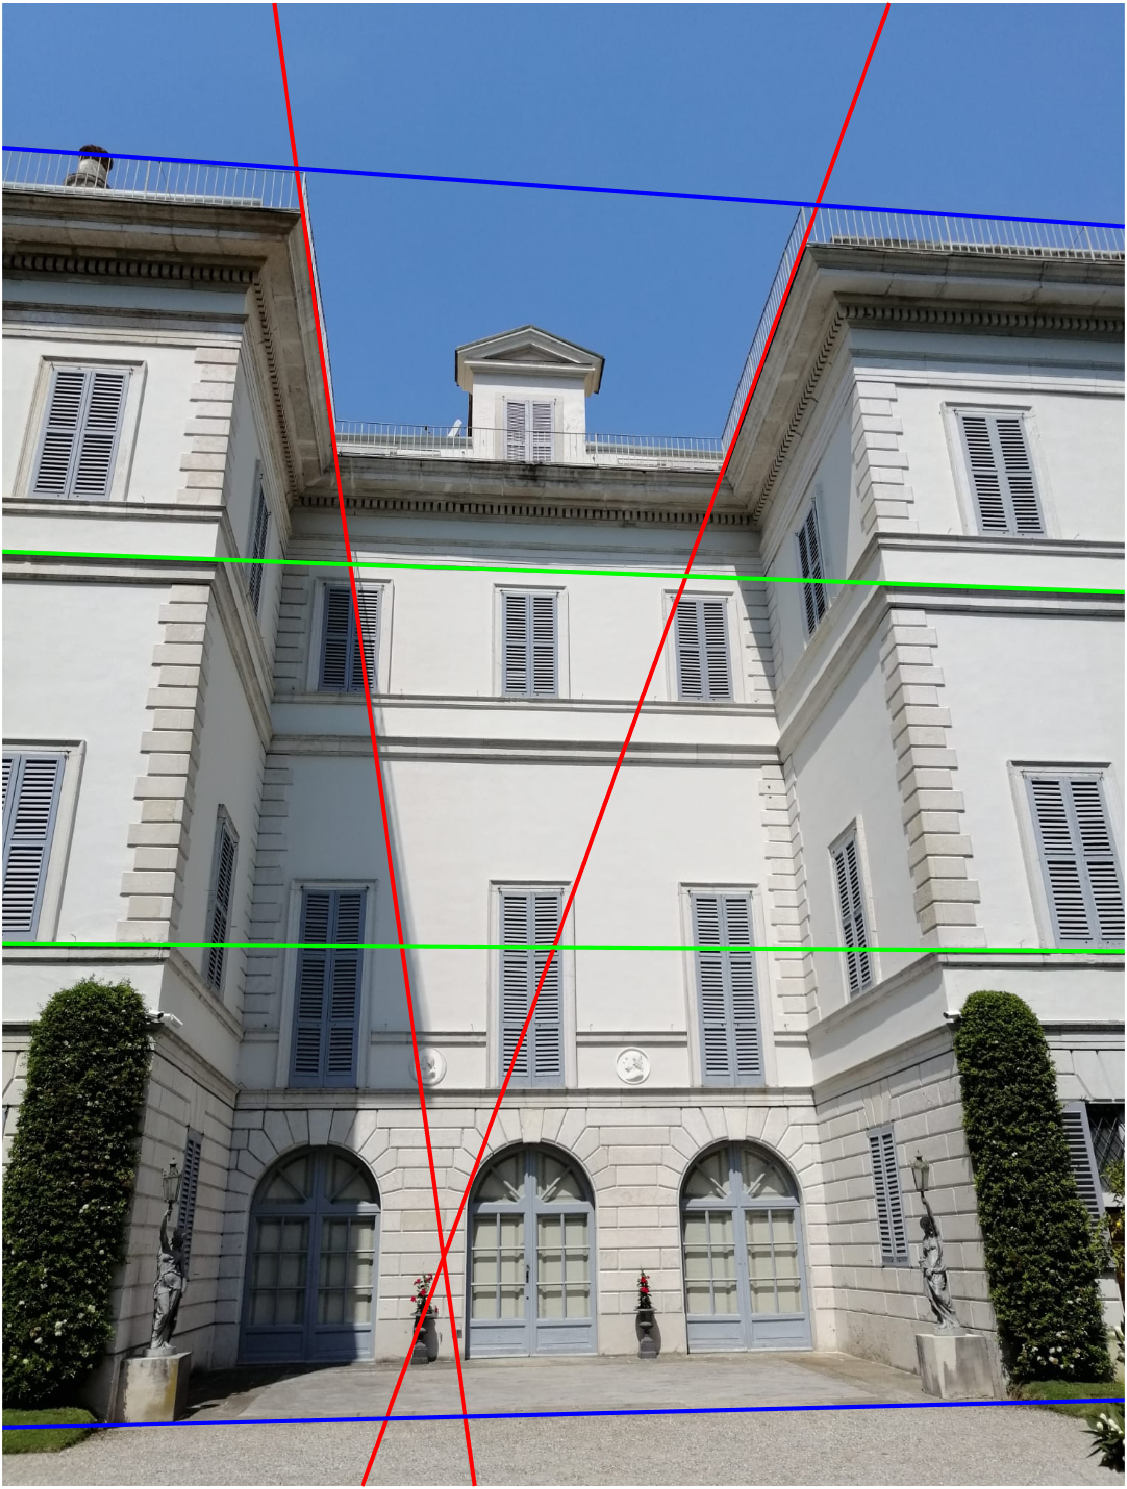
\includegraphics[width=0.4\textwidth]{output/G1_lines.png}
    }
    \quad
    \subfloat[Affine rectified image\label{fig:g1_affine_rectified}]{
        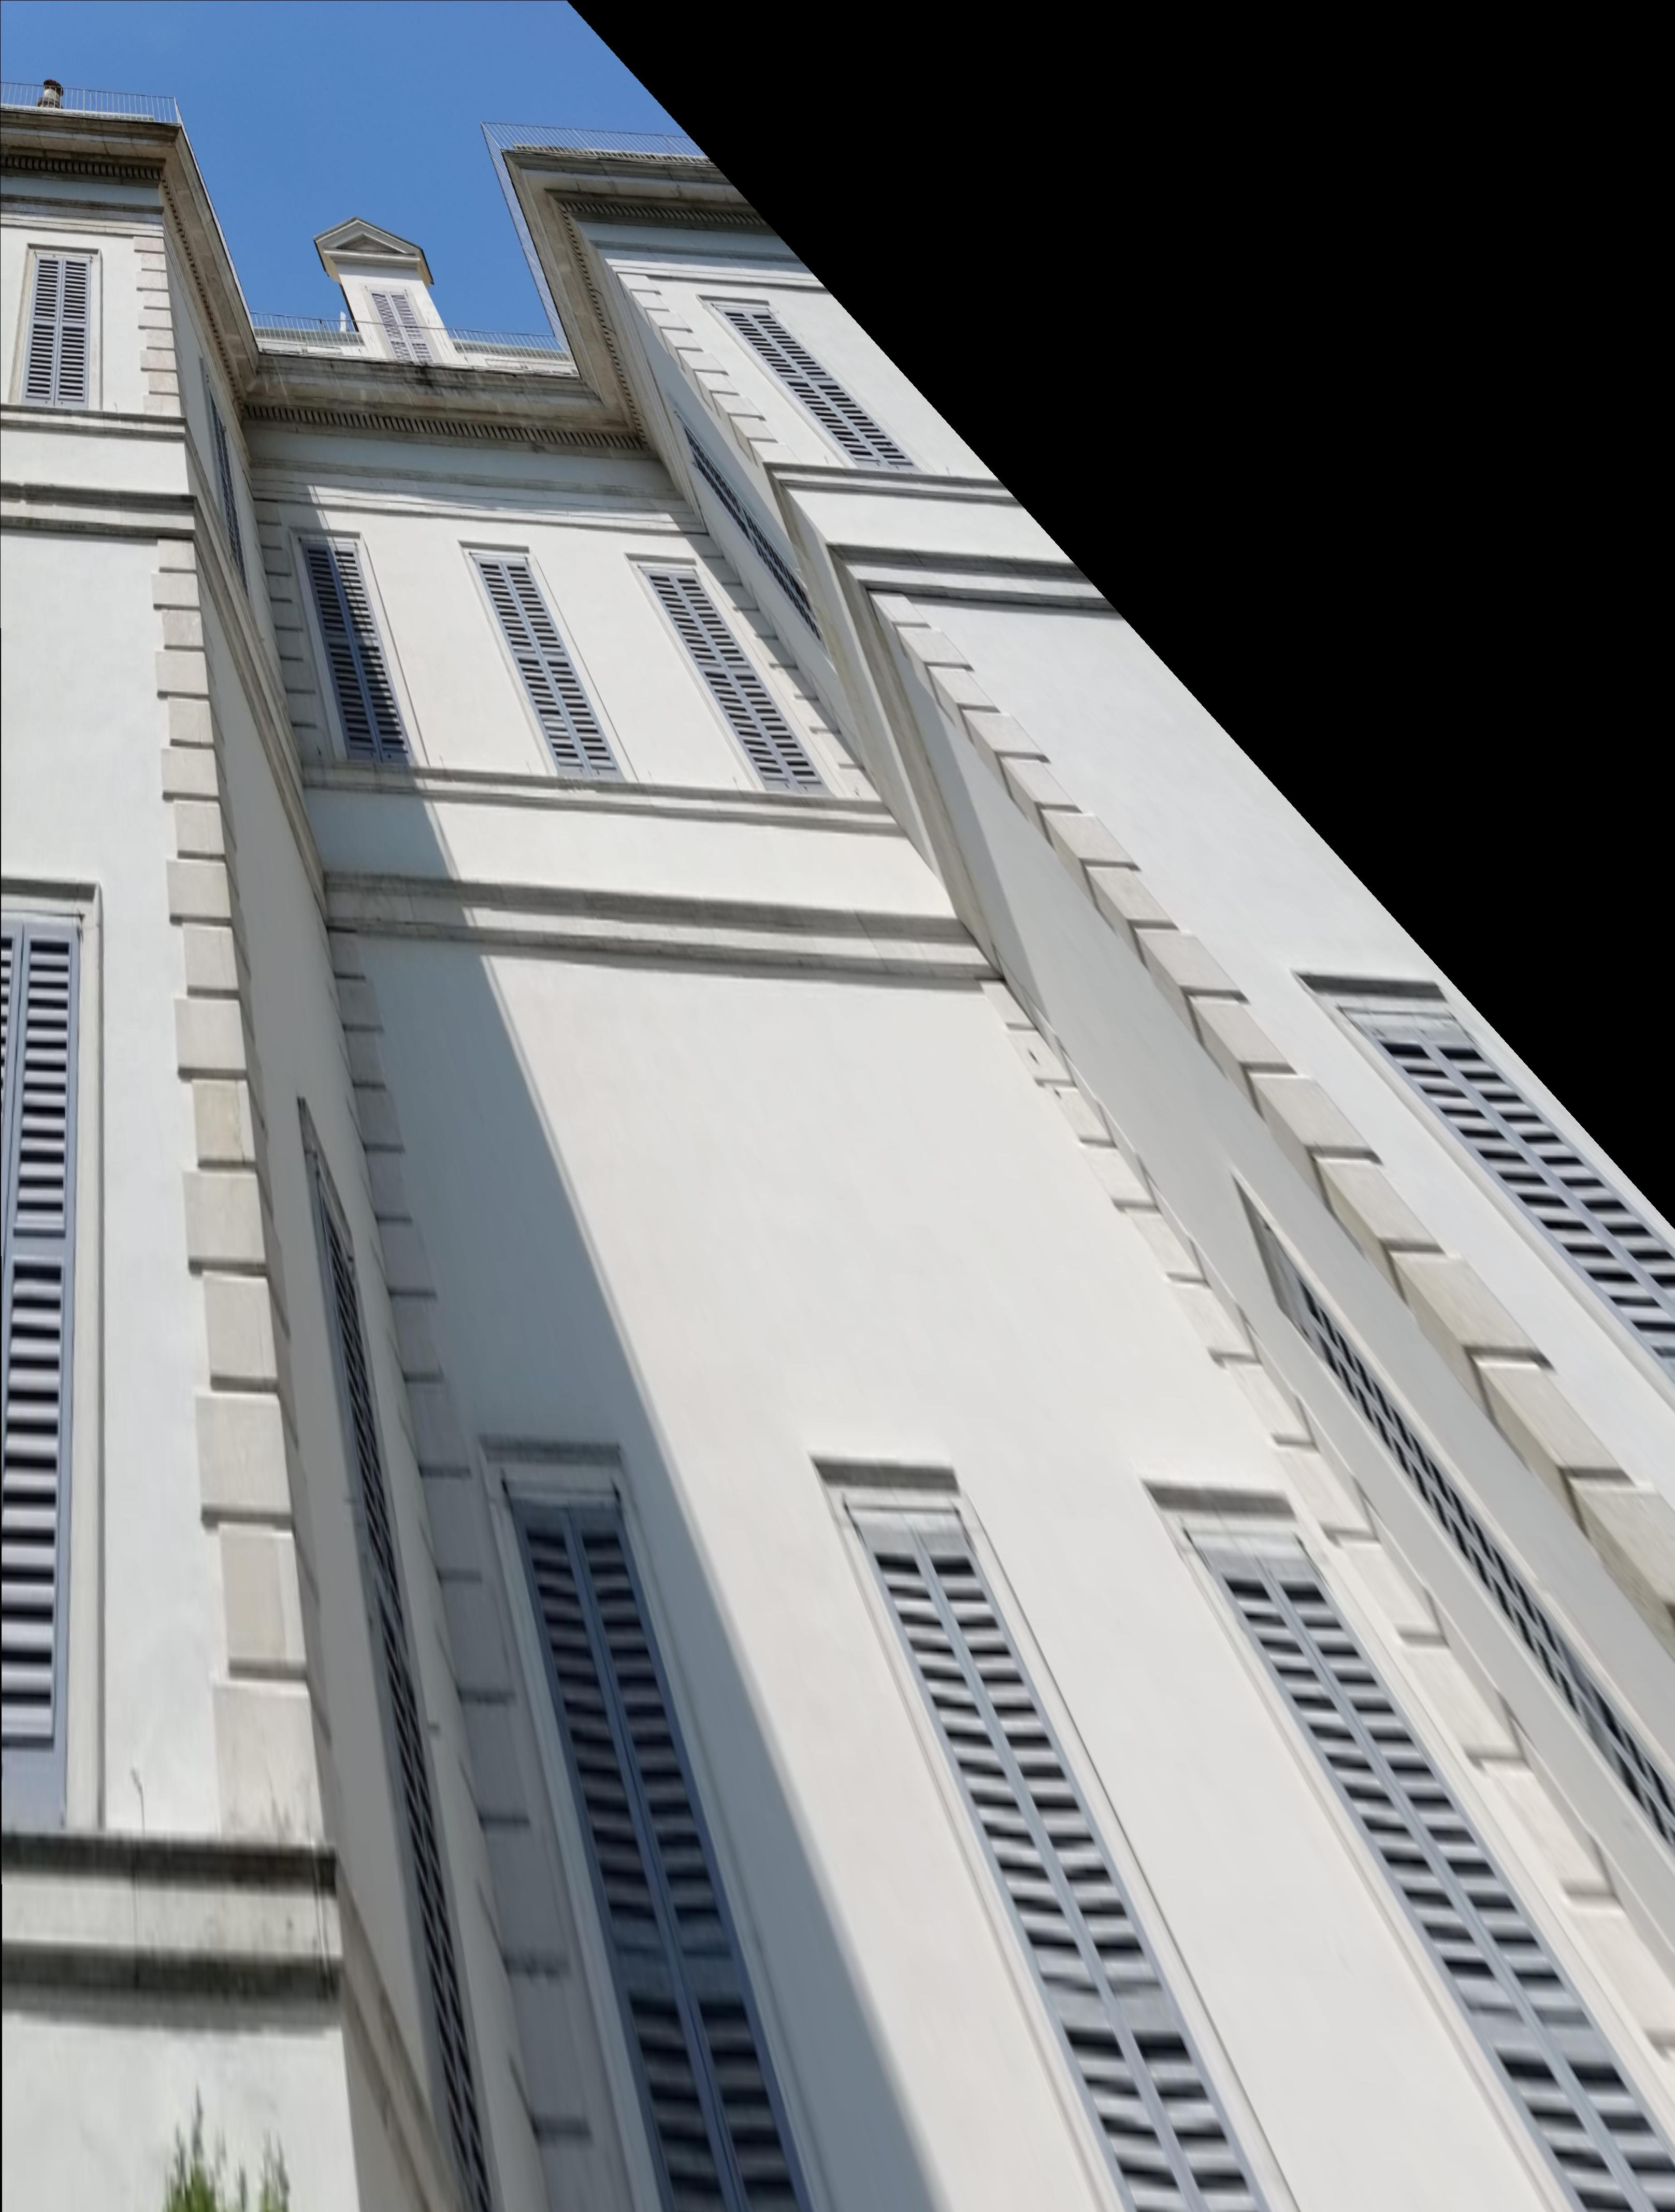
\includegraphics[width=0.4\textwidth]{output/G1_affine.jpg}
    }
    \caption{Affine rectification of the Villa image}
    \label{fig:g1_affine}
\end{figure}

It is crucial to select the red lines in figure \ref{fig:g1_affine_lines}, as we want those lines to be parallel in the output.

\section{Metric rectification}
Now that we have the affine rectified image, we need two more constraints to compute the image of $C^{*'}_\infty$. In particular, we can use two pairs of lines at known angles, remembering the equation:

\[
\cos\theta = \frac{l^{'T}\,C^{*'}_\infty\,m^{'}}{\sqrt{(l^{'T}\,C^{*'}_\infty\,l^{'})\,(m^{'T}\,C^{*'}_\infty\,m^{'})}}
\]

Since the assignment specifies the \textbf{position of the sun}, we can use this information along with the shadows in the image for the first constraint, and use two orthogonal lines for the remaining unknown.

\begin{minted}{matlab}
cosTheta = cos(atan(3.9));
orthogonalLines = drawLines('Draw orthogonal lines', 2, 'r');
angledLines = drawLines('Draw an horizontal line and the shadow', 2, 'g');
\end{minted}
\newpage

Finally, we can solve the system of equation with these two constraints to find the metric rectification matrix $H_{metric}$ (or rather, its inverse, since we need to multiply it with $H_{aff}$ and Matlab suggests to use the \verb|\| operator as it is faster):

\begin{minted}{matlab}
% Solve the system using the selected lines
syms x1 x2;
imDCCP = [x1,x2,0;x2,1,0;0,0,0];
orthogonalConstraintEq = a.'*imDCCP*b == 0;
angledConstraintEq = cosTheta*sqrt((l.'*imDCCP*l)*(m.'*imDCCP*m)) ...
	== (l.'*imDCCP*m);
S = solve([orthogonalConstraintEq, angledConstraintEq], [x1, x2]);

% Note that, depending on the selected lines, 1 or two solutions
% could be returned. Here, the case with 1 solution is handled.
s1 = double(S.x1(1));
s2 = double(S.x2(1));

% Build the matrix via Cholesky decomposition
K = chol([s1, s2; s2, 1]);
H_metric_inv = [K.',[0;0];0,0,1];
\end{minted}

Finally, we compute the rectification matrix and apply it to the image. The output size is scaled by a factor of 5 to show a larger portion of the image.

\begin{minted}{matlab}
Hrect = H_metric_inv \ H_aff;
tform = projective2d(Hrect.');
imgRect = im2double(imwarp(img, tform, 'OutputView', imref2d(size(img)*5)));
figure; imshow(imgRect);
\end{minted}

\[
H_{rect} \approx
\begin{pmatrix}
1.0051 & 0 & 0\\
-0.4713 & 1.1045 & 0\\
\num{-1.2015e-5} & \num{-8.2565e-4} & 1
\end{pmatrix}
\]

\begin{figure}[H]
    \centering
    \subfloat[Lines used for metric rectification\label{fig:g1_metric_lines}]{
        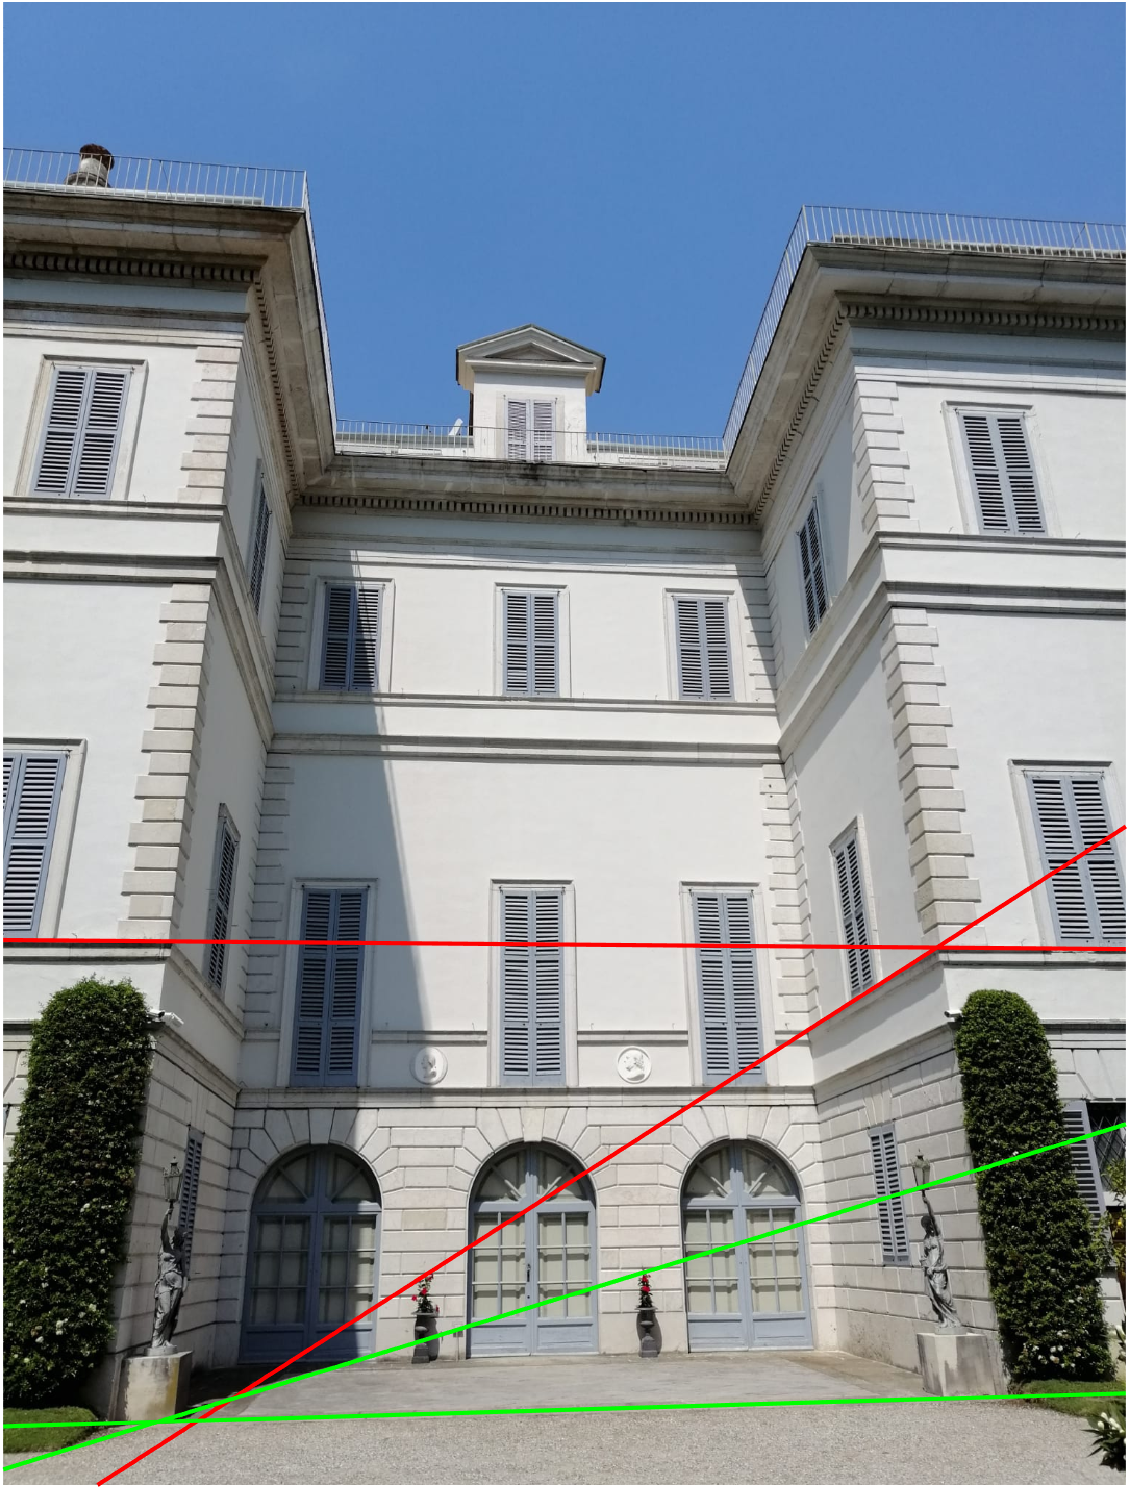
\includegraphics[width=0.4\textwidth]{output/G1_lines_metric.png}
    }
    \quad
    \subfloat[Metric rectified image\label{fig:g1_metric_rectified}]{
        \includegraphics[width=0.4\textwidth]{output/G1_metric.png}
    }
    \caption{Metric rectification lines and result}
    \label{fig:g1_metric}
\end{figure}

Even though the metric rectification does not show the full horizontal section, it is enough for our goal of calculating the ratio between facades.

\section{Ratio between facades 2 and 3}

To calculate the ratio, we need to find the length of each facade. This can be done by simply selecting the corners of each facade (so three points in total since they share one corner) and calculating the distance between the points.

For better precision, instead of selecting the points in the metric rectified image we can select them on the original image and multiply $H_{rect}$ to get their images.

\begin{minted}{matlab}
% Select three points
[x,y] = getpts();
% Convert to homogeneous coords and apply the transform
xyRect = Hrect * [x y [1;1;1]].';
% Normalize the transformed points (for accuracy and easier plotting)
xyRect = xyRect ./ xyRect(3, :); 	
\end{minted}

\begin{figure}[H]
    \centering
    \subfloat[Points selected in the original image\label{fig:g1_ratio_points_orig}]{
        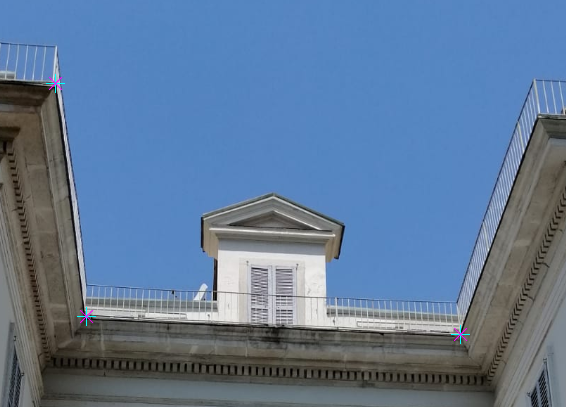
\includegraphics[width=0.4\textwidth]{output/G1_ratio_pts.png}
    }
    \quad
    \subfloat[Image of the points in the warped image\label{fig:g1_ratio_points_warped}]{
        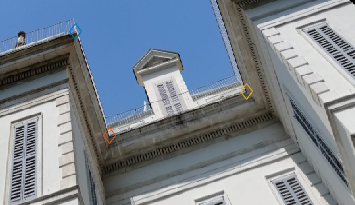
\includegraphics[width=0.4\textwidth]{output/G1_ratio_pts_warped.png}
    }
    \caption{Points selected for the facade length calculation}
    \label{fig:g1_ratio_points}
\end{figure}

We can then calculate the length (remember the points are normalized, so by subtracting them we effectively get rid of the $w$ coordinate and consider them points in the cartesian plane) and print the ratio.

\begin{minted}{matlab}
p2 = xyRect(:,1);
p23 = xyRect(:,2);
p3 = xyRect(:,3);
lengthF2 = norm(p23-p2);
lengthF3 = norm(p3-p23);
fprintf('Ratio of facade 2 over 3: %d\n', lengthF2 / lengthF3);
\end{minted}

With the above points, the obtained ratio is $\approx$ 65\%.

\chapter{G2 - Calibration}

We now want to find the calibration matrix $\mathbf{K}$ containing the intrinsic parameters of the camera. From the assignment, we know the skew factor is null, thus there are four unknowns, so we will need four equations to find $\mathbf{K}$.

Since we already have $H_{rect}$ from the previous step, we can use the direct method to calibrate from a rectified face plus orthogonal vanishing points. The equations are:

\begin{equation}
	\begin{cases}
		\mathbf{l^{'}_\infty} = \omega\,\mathbf{v}\\
		h_1^T\,\omega\,h_2 = 0\\
		h_1^T\,\omega\,h_1 - h_2^T\,\omega\,h_2 = 0\\
	\end{cases}
\end{equation}

The Matlab code is pretty straightforward:

\begin{minted}{matlab}
%% Get the vertical vanishing point
verticalLines = drawLines('Draw vertical parallel lines', 2, 'r');
vpV = hpnorm(cross(verticalLines(1,:), verticalLines(2,:)));
%% Find two more vanishing points
horizontalLines = drawLines('Draw two lines on the horizontal plane', 2, 'g');
vp1 = hpnorm(cross(horizontalLines(1,:), imHLinf));
vp2 = hpnorm(cross(horizontalLines(2,:), imHLinf));	
%% Compute the IAC
Hrect_inv = inv(Hrect);
h1 = hpnorm(Hrect_inv(:,1));
h2 = hpnorm(Hrect_inv(:,2));

syms x1 x2 x3 x4;
x = [x1 0 x2; 0 1 x3; x2 x3 x4];
\end{minted}
\newpage
\begin{minted}{matlab}
S = solve([
    vp1 * x * vpV.' == 0;
    vp2 * x * vpV.' == 0;
    h1.' * x * h2 == 0;
    h1.' * x * h1 == h2.' * x * h2
], [x1 x2 x3 x4]);
s1 = double(S.x1); s2 = double(S.x2);
s3 = double(S.x3); s4 = double(S.x4);
omega = [s1 0 s2; 0 1 s3; s2 s3 s4];
\end{minted}

The result is the following (image size is normalized to 1):

\[
\mathbf{K} =
\begin{pmatrix}
f_x & 0 & U_o\\
0 & f_y & V_o\\
0 & 0 & 1
\end{pmatrix}
\approx
\begin{pmatrix}
0.9160 & 0 & 0.4797\\
0 & 0.8099 & 0.4913\\
0 & 0 & 1
\end{pmatrix}
\]


Camera intrinsic parameters:
\begin{itemize}
\item \textbf{Aspect ratio}: $\alpha = \frac{f_x}{f_y} \approx 1.1310$
\item \textbf{Focal distance}: $f_x \approx 0.9160$, $f_y \approx 0.8099$
\item \textbf{Principal point}: $(U_o, V_o) \approx (0.4797, 0.4913)$
\end{itemize}

\chapter{G3 - Reconstruction of a vertical facade}

Now that we have the $\omega$ matrix, we can use it to rectify facade 3. By intersecting it with the line at the infinity of the vertical plane (which we can find using two families of parallel lines, as before) we obtain the image of $\mathbf{I}$ and $\mathbf{J}$ and compute the image of the dual conic. We can then use \verb|svd| to retrieve the $\mathbf{U}$ matrix, which is the transpose of the rectifying homography. However, the following equation is used for improved accuracy:

\[
H_{rect}^{-1} = U\,\begin{pmatrix}
\sqrt{s1} & 0 & 0\\
0 & \sqrt{s2} & 0\\
0 & 0 & \epsilon
\end{pmatrix}
\]

Here are the most important parts of the code:

\begin{minted}{matlab}
%% Find the intersection between the line at infinity and the IAC
syms x1 x2;
x = [x1 x2 1].';
S = solve([
    imVLinf.' * x == 0, ...
    x.' * omega * x == 0
], [x1,x2]);
s1 = double(S.x1);
s2 = double(S.x2);
%% Compute the rectification matrix for the vertical facade
I = [s1(1) s2(1) 1].'; J = [s1(2) s2(2) 1].';
imDCCP2 = I*(J.')+J*(I.');
imDCCP2 = imDCCP2 ./ norm(imDCCP2);
[U, S2, ~] = svd(imDCCP2);
S2(3,3) = 1;
Hrect2_inv = U * sqrt(S2);
\end{minted}

If we try to display the image now, it will be upside down. We can try to fix this by using one of the lines we selected earlier, computing its image and calculating its rotation.

\begin{minted}{matlab}
hLineRot = Hrect2_inv.' * parallelLines{2}(1,:).';
rotAngle = atan(-hLineRot(1)/hLineRot(2)) + pi;
Hrot = buildRotationMatrix(-rotAngle);
\end{minted}

\begin{figure}[H]
    \centering
    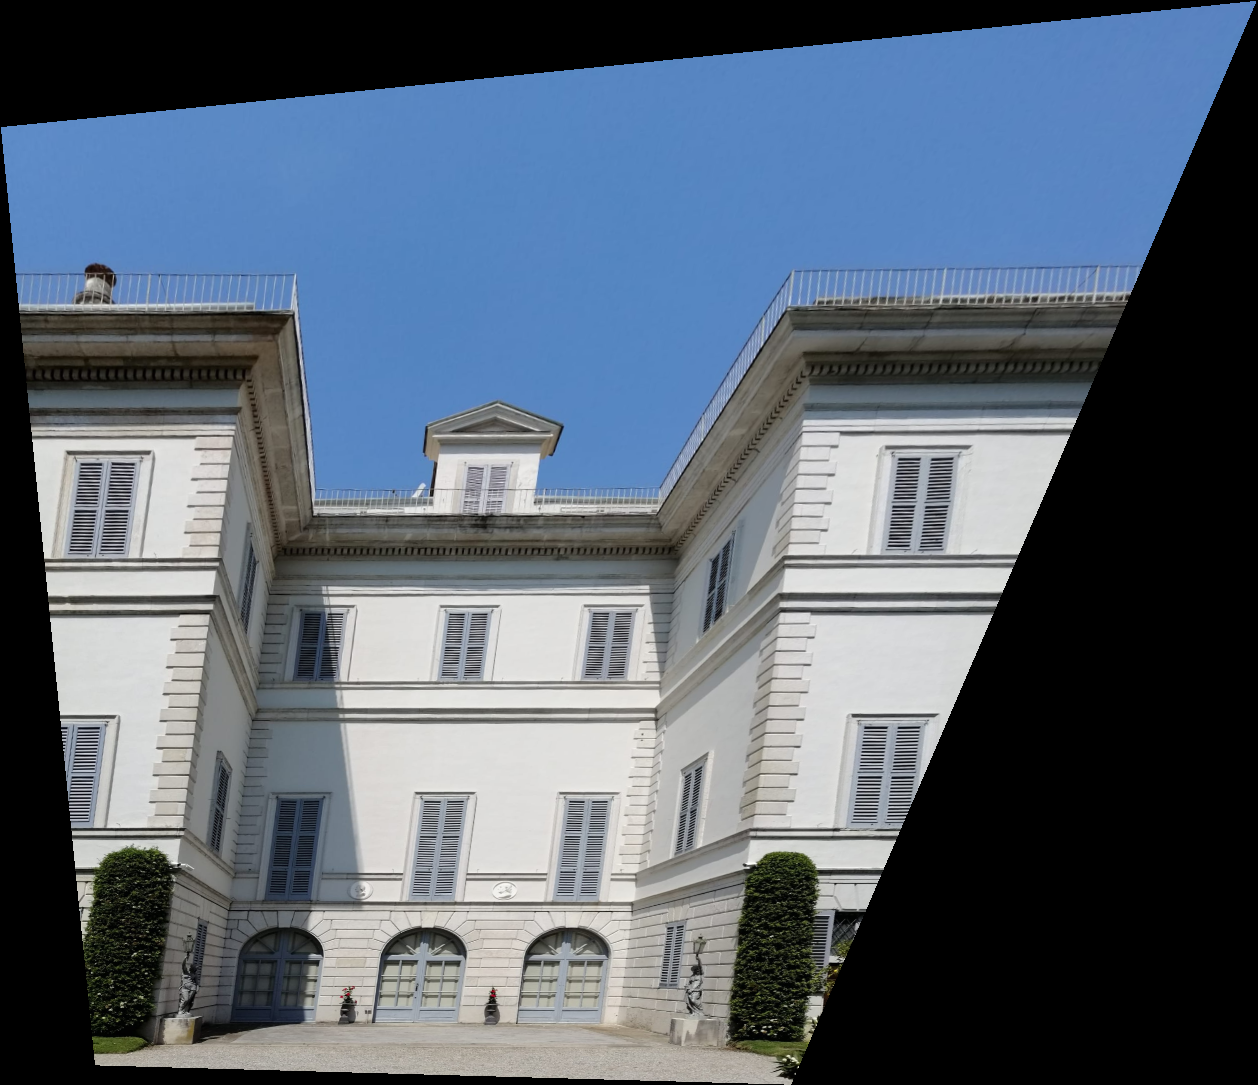
\includegraphics[width=0.8\textwidth]{output/G3_final.png}
    \caption{Rectified vertical facade}
    \label{fig:g3_rectified}
\end{figure}

\chapter{G4 - Localization}

The last part of the assignment asks for the relative pose between facade 3 and the camera reference.
To accomplish this, we can use the $\mathbf{K}$ matrix and a planar surface: by fitting an homography that transforms the plane in the image to a new reference frame defined by us (which will be the camera reference frame), we can determine the position of the camera itself.

The new reference frame $\pi$ can be identified with its versors $[i_\pi, j_\pi, k_\pi]$ and the origin $o_\pi$. To find these, we first need to identify the homography.

Our plane will be the bottom horizontal plane (\ref{fig:g4_points}). From G1 we know the ratio \verb|ratio| between facades 2 and 3, which we can use to place these points in the new reference plane. Starting from the bottom left corner, points will be mapped like this:
\begin{minted}{matlab}
points_c = [0 0; 0 ratio; 1 ratio; 1 0];	
\end{minted}

After selecting the points in the image (\verb|points_img|), we use the \verb|fitgeotrans| function to fit the homography:
\begin{minted}{matlab}
tform_loc = fitgeotrans(points_c, points_img, 'projective');
H_loc = tform_loc.T;
\end{minted}

The following relation holds:
\[
[i_\pi, j_\pi, o_\pi] = \mathbf{K^{-1}}H_{loc}
\]
so we use it to find all parameters (remembering $k_\pi = i_\pi \times j_\pi$):
\begin{minted}{matlab}
c_ref = K \ H_loc;
c_ref = c_ref ./ c_ref(3,:);
R = [c_ref(:,1), c_ref(:,2), cross(c_ref(:,1), c_ref(:,2))];
[U, ~, V] = svd(R);
R = U * V';
\end{minted}
Notice how each column of the \verb|c_ref| matrix is normalized; this is to avoid numerical errors. The \verb|svd| is needed because the $\mathbf{R}$ matrix is not exactly orthogonal, also due to numerical errors.

We can now decompose calculate the camera orientation and position like this:
\begin{minted}{matlab}
camera_orientation = R.';
camera_pos = -R.' * c_ref(:,3);	
\end{minted}

The only thing left to do is solve for scale using the provided camera height of 1.5m.
\begin{minted}{matlab}
camera_mult = camera_pos(3) / 1.5;
camera_pos_m = camera_pos ./ camera_mult;
points_c_m = points_c ./ camera_mult;	
\end{minted}

The resulting locations of the points in the camera reference frame are $(0, 0)$, $(0, 10.25)$, $(15.77, 10.25)$, $(15.77, 0)$. Position of the camera itself is $(5.86, -17.8, 1.50)$.

The orientation is:
\begin{verbatim}
 0.9280    0.3304    0.1721
-0.2321    0.1513    0.9608
 0.2914   -0.9316    0.2171
\end{verbatim}

To see the position and orientation of the camera, we can use the Matlab functions \verb|plotCamera| and \verb|pcshow| which render the camera itself and the points in a 3D space. I have also added a rectangle representing facade 3 to better understand the positioning of the camera (not actual height).

\begin{figure}[H]
    \centering
    \subfloat[Selected points\label{fig:g4_points}]{
        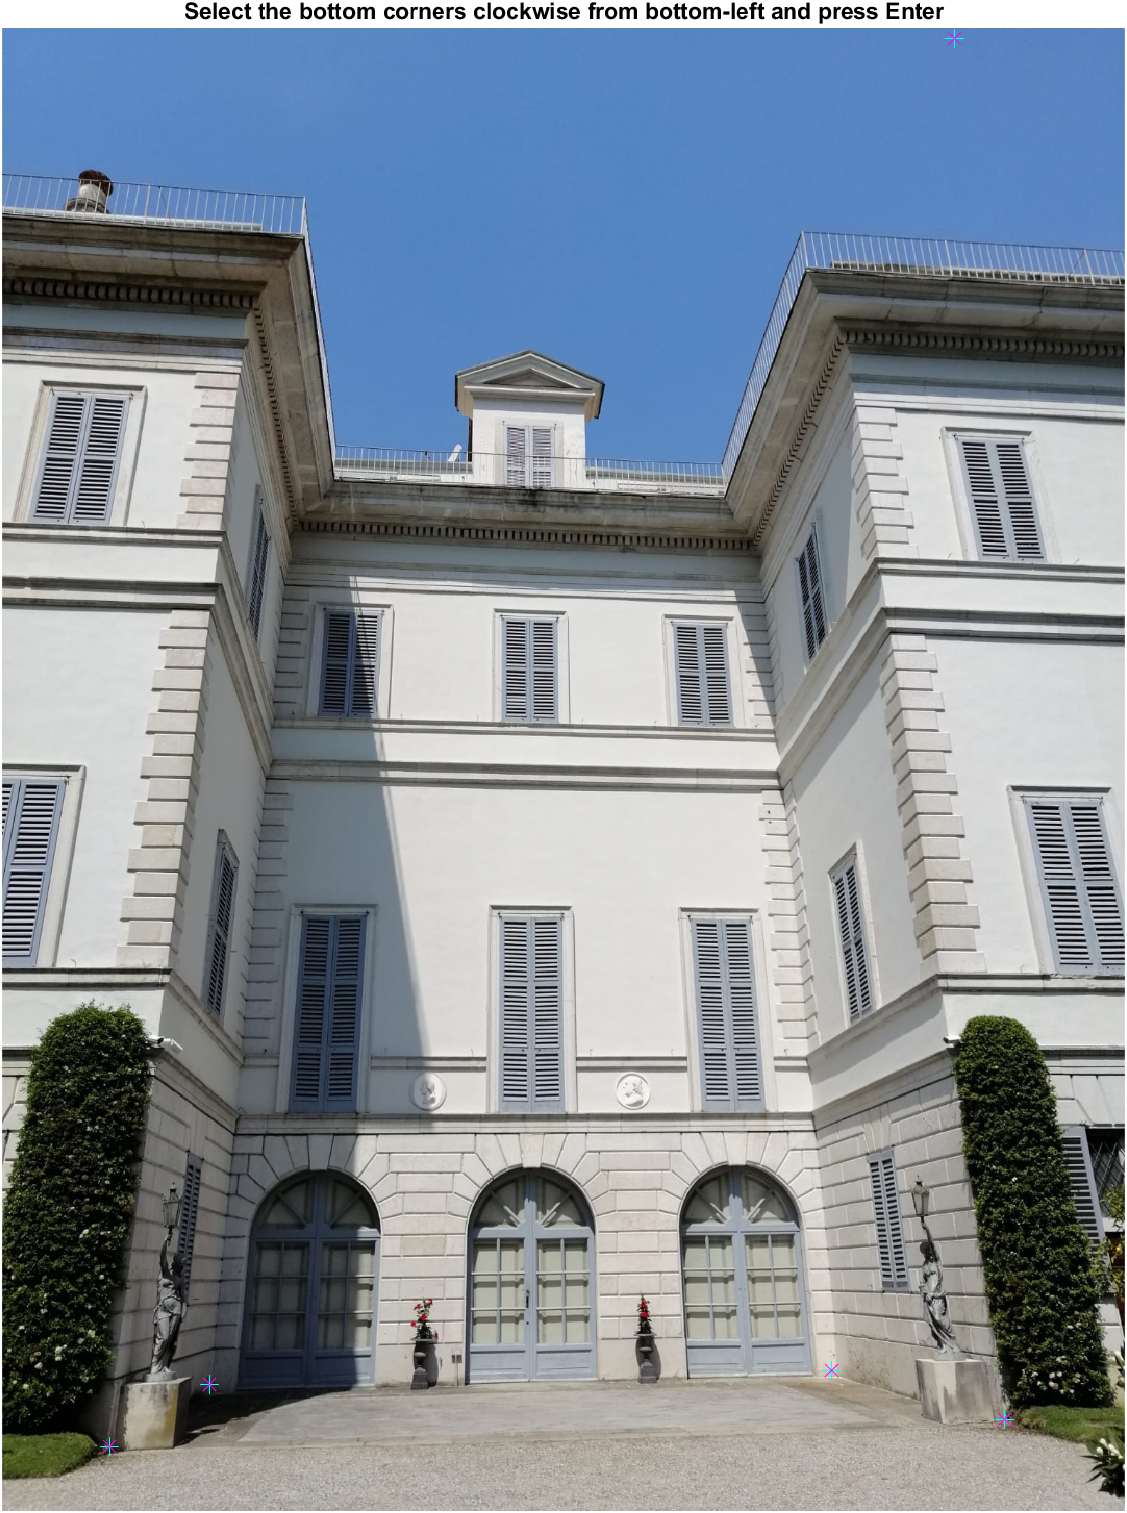
\includegraphics[width=0.4\textwidth]{output/G4_points.png}
    }
    \quad
    \subfloat[The relative camera pose\label{fig:g4_result}]{
        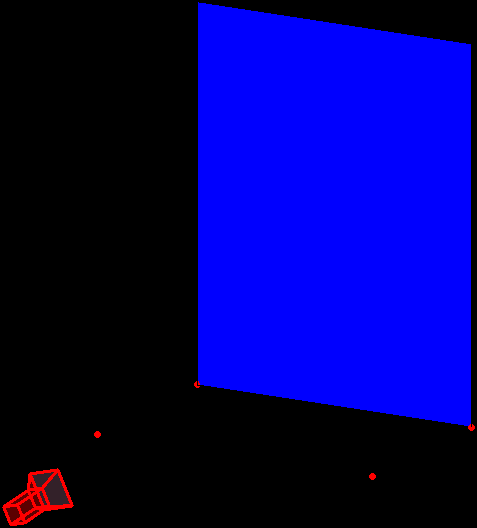
\includegraphics[width=0.4\textwidth]{output/G4_camera.png}
    }
    \caption{Selected lines and results of the localization process}
    \label{fig:g4_images}
\end{figure}

%-------------------------------------------------------------------------
%   BIBLIOGRAPHY
%-------------------------------------------------------------------------

\addtocontents{toc}{\vspace{2em}} % Add a gap in the Contents, for aesthetics
%\bibliography{Thesis_bibliography} % The references information are stored in the file named "Thesis_bibliography.bib"

%-------------------------------------------------------------------------
%   APPENDICES
%-------------------------------------------------------------------------

\addtocontents{toc}{\vspace{2em}} % Add a gap in the Contents, for aesthetics
\appendix
\chapter{Matlab functions}
\label{appendix:functions}

\begin{minted}{matlab}
function [l] = segToLine(pts)
a = [pts(1,:)';1];
b = [pts(2,:)';1];
l = cross(a,b);
l = l./norm(l);
end

function [C, dist] = fitLine(XY)
  [rows,npts] = size(XY);
  if npts < 2
      error('Too few points to fit line');
  end
  if rows == 2
    XY = [XY; ones(1,npts)];
  end
  if npts == 2
    XY = [XY zeros(3,1)]; 
  end
  [XYn, T] = normalise2dpts(XY);
  [u d v] = svd(XYn',0);
  C = v(:,3);
  C = T'*C;
  if nargout==2   
      dist = abs(C(1)*XY(1,:) + C(2)*XY(2,:) + C(3));
  end
end
\end{minted}
\newpage
\begin{minted}{matlab}
function lines = drawLineFamilies(title, nFamilies, nLinesPerFamily)
    colors = 'rgbm';
    lines = cell(nFamilies, 1); % store lines
    for i = 1:nFamilies
        lines{i} = drawLines([title, ' - family ', num2str(i), ' of ', ...
        	num2str(nFamilies)], nLinesPerFamily, colors(i));
    end
end

function lines = drawLines(title_, nLines, color)
    count = 1;
    lines = nan(nLines, 3);
    while(count <= nLines)
        figure(gcf);
        title([title_, ' - segment ', num2str(count), ' of ', num2str(nLines)]);
        segment = drawline('Color', color);
        lines(count, :) = hpnorm(segToLine(segment.Position));
        count = count + 1;
    end
end

% Normalize a point in homogeneous coordinates.
function p_norm = hpnorm(p)
    p_norm = p ./ p(3);
end
\end{minted}
\newpage
\begin{minted}{matlab}
function [H, imLinf] = buildHaff(lines)
    V = nan(2, length(lines));
    for i = 1:length(lines)
        A = lines{i}(:,1:2);
        B = -lines{i}(:,3);
        V(:,i) = A\B;
    end
    imLinf = hpnorm(fitLine(V));
    H = [eye(2), zeros(2,1); imLinf(:).'];
end

function matrix = buildRotationMatrix(angle)
    ca = cos(angle);
    sa = sin(angle);
    matrix = [ca,-sa,0;sa,ca,0;0,0,1];
end	
\end{minted}


% LIST OF FIGURES
{\hypersetup{linkcolor=black}
\listoffigures
}

\end{document}
